\documentclass[11pt]{article}
\usepackage[letterpaper,margin=1in]{geometry}
\usepackage{times}
\usepackage{graphicx}
\usepackage{amsmath}
\usepackage{amssymb}
\usepackage{hyperref}
\usepackage{natbib}

\graphicspath{{figures/}}

\title{\bf Unexpected Pitfalls in Deep Neural Sequence Models}
\author{
    An Ambitious Researcher \\
    Department of AI \\
    Some Institute \\
    \texttt{researcher@institute.edu}
}
\date{}

\begin{document}

\maketitle

\begin{abstract}
Although recent advances in deep learning have yielded impressive results on benchmark tasks, real-world deployments often expose subtle pitfalls. We study neural sequence models under various training and deployment conditions, observing unexpected behaviors, such as degraded generalization when scaling pretraining datasets and inconsistent validation trends induced by certain architectural choices. These findings highlight fragile behaviors and suggest that prevailing best practices might benefit from revisiting certain standard assumptions.
\end{abstract}

\section{Introduction}
Deep learning has achieved state-of-the-art performance in language, vision, and multimodal domains \citep{lecun2015}. Despite these successes, reports of negative or inconclusive results often remain unpublished. However, real-world adoption involves conditions that deviate from clean benchmark assumptions, leading to unexpected performance drops, complicated training patterns, and reliability issues. By scrutinizing neural sequence models with small but carefully designed experiments, we expose nuances that point to potential root causes of fragile generalization. These insights illuminate hidden execution or architectural details that can hinder robust performance and motivate further community exploration.

Here, we examine pitfalls in common sequence modeling pipelines, comparing baseline architectures with variations in pretraining, freezing encoder layers, and removing positional embeddings. Our contributions are twofold. First, we show that adding more pretraining data does not always guarantee better validation metrics. Second, we highlight how architectural modifications can yield mixed or deteriorating results, demonstrated through confusion matrices and ablation checks. These observations emphasize that a systematic approach to negative and inconclusive findings is essential for refining deep learning methodologies.

\section{Related Work}
Recent literature underscores the prevalence of subtle pitfalls that arise from partial or uneven training improvements. \citet{simonyan2015} note diminishing returns when scaling network depth without careful parameter initialization. \citet{vaswani2017} suggest attention-based models outperform convolutions, yet inconsistencies in real deployments persist. Across domains, inconclusive or negative results often remain confined to supplemental materials. Our work continues this discussion by detailing experimental instabilities and proposing explicit demonstration of these issues.

\section{Method / Problem Discussion}
We adopt a standard neural sequence encoder-decoder framework, varying configurations to investigate how each component contributes to success or failure. Architecturally, the baseline uses an attention-based transformer with a projection head for classification tasks. We augment data modestly but test the hypothesis that more pretraining data always boosts performance. At each stage, we measure metrics such as macro-F1 and confusion across classes.

Positional embeddings, freezing the encoder, and removing the projection head are known modifications. Our experiments confirm that while removing these components can simplify training, it can also reduce accuracy or negatively affect confusion patterns. These choices highlight the complexity of real-world neural modeling, suggesting that conventional wisdom may not always hold.

\section{Experiments}
We first examine the baseline model. Figure~\ref{fig:main1} shows macro-F1 and loss curves across epochs. Counter to expectations, the validation score briefly improves then plateaus, indicating limited benefit from additional pretraining. Figure~\ref{fig:main2} compares the final validation metrics with a corresponding confusion matrix. Although classification is generally strong, certain classes remain confused, revealing that more training data does not always eradicate misclassification.

\begin{figure}[t]
\centering
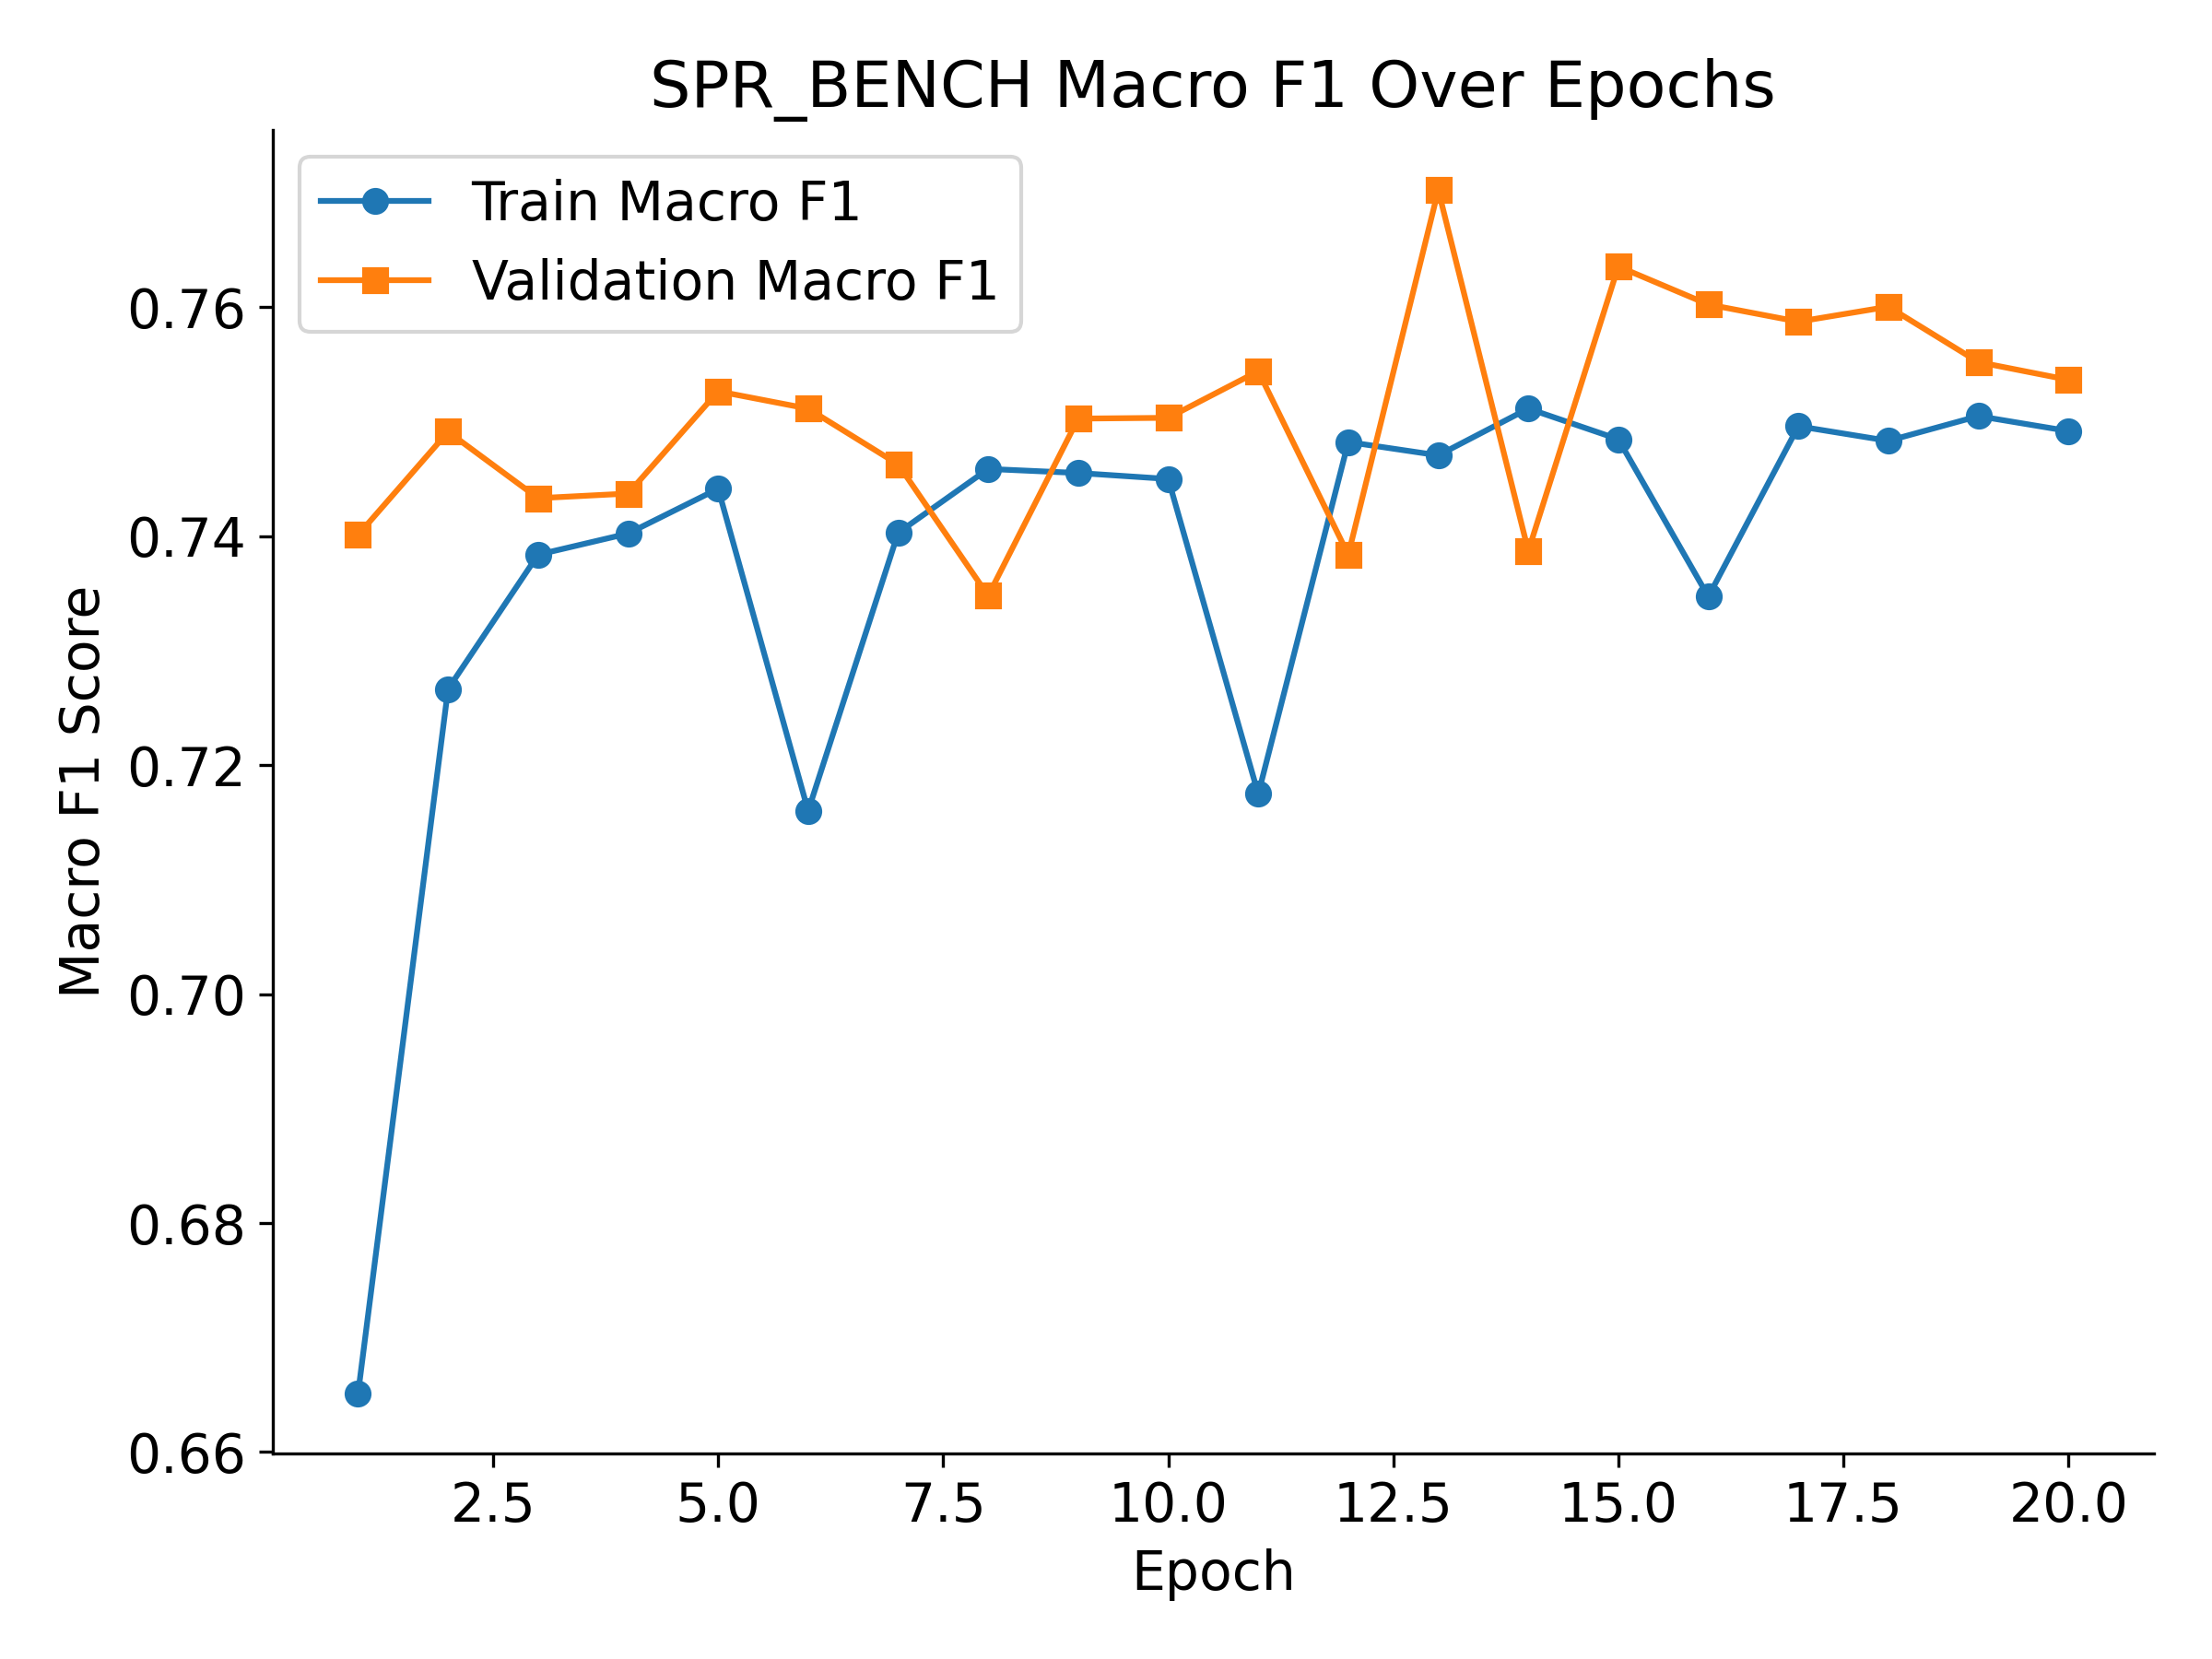
\includegraphics[width=0.45\textwidth]{baseline_macro_F1.png}
\hfill
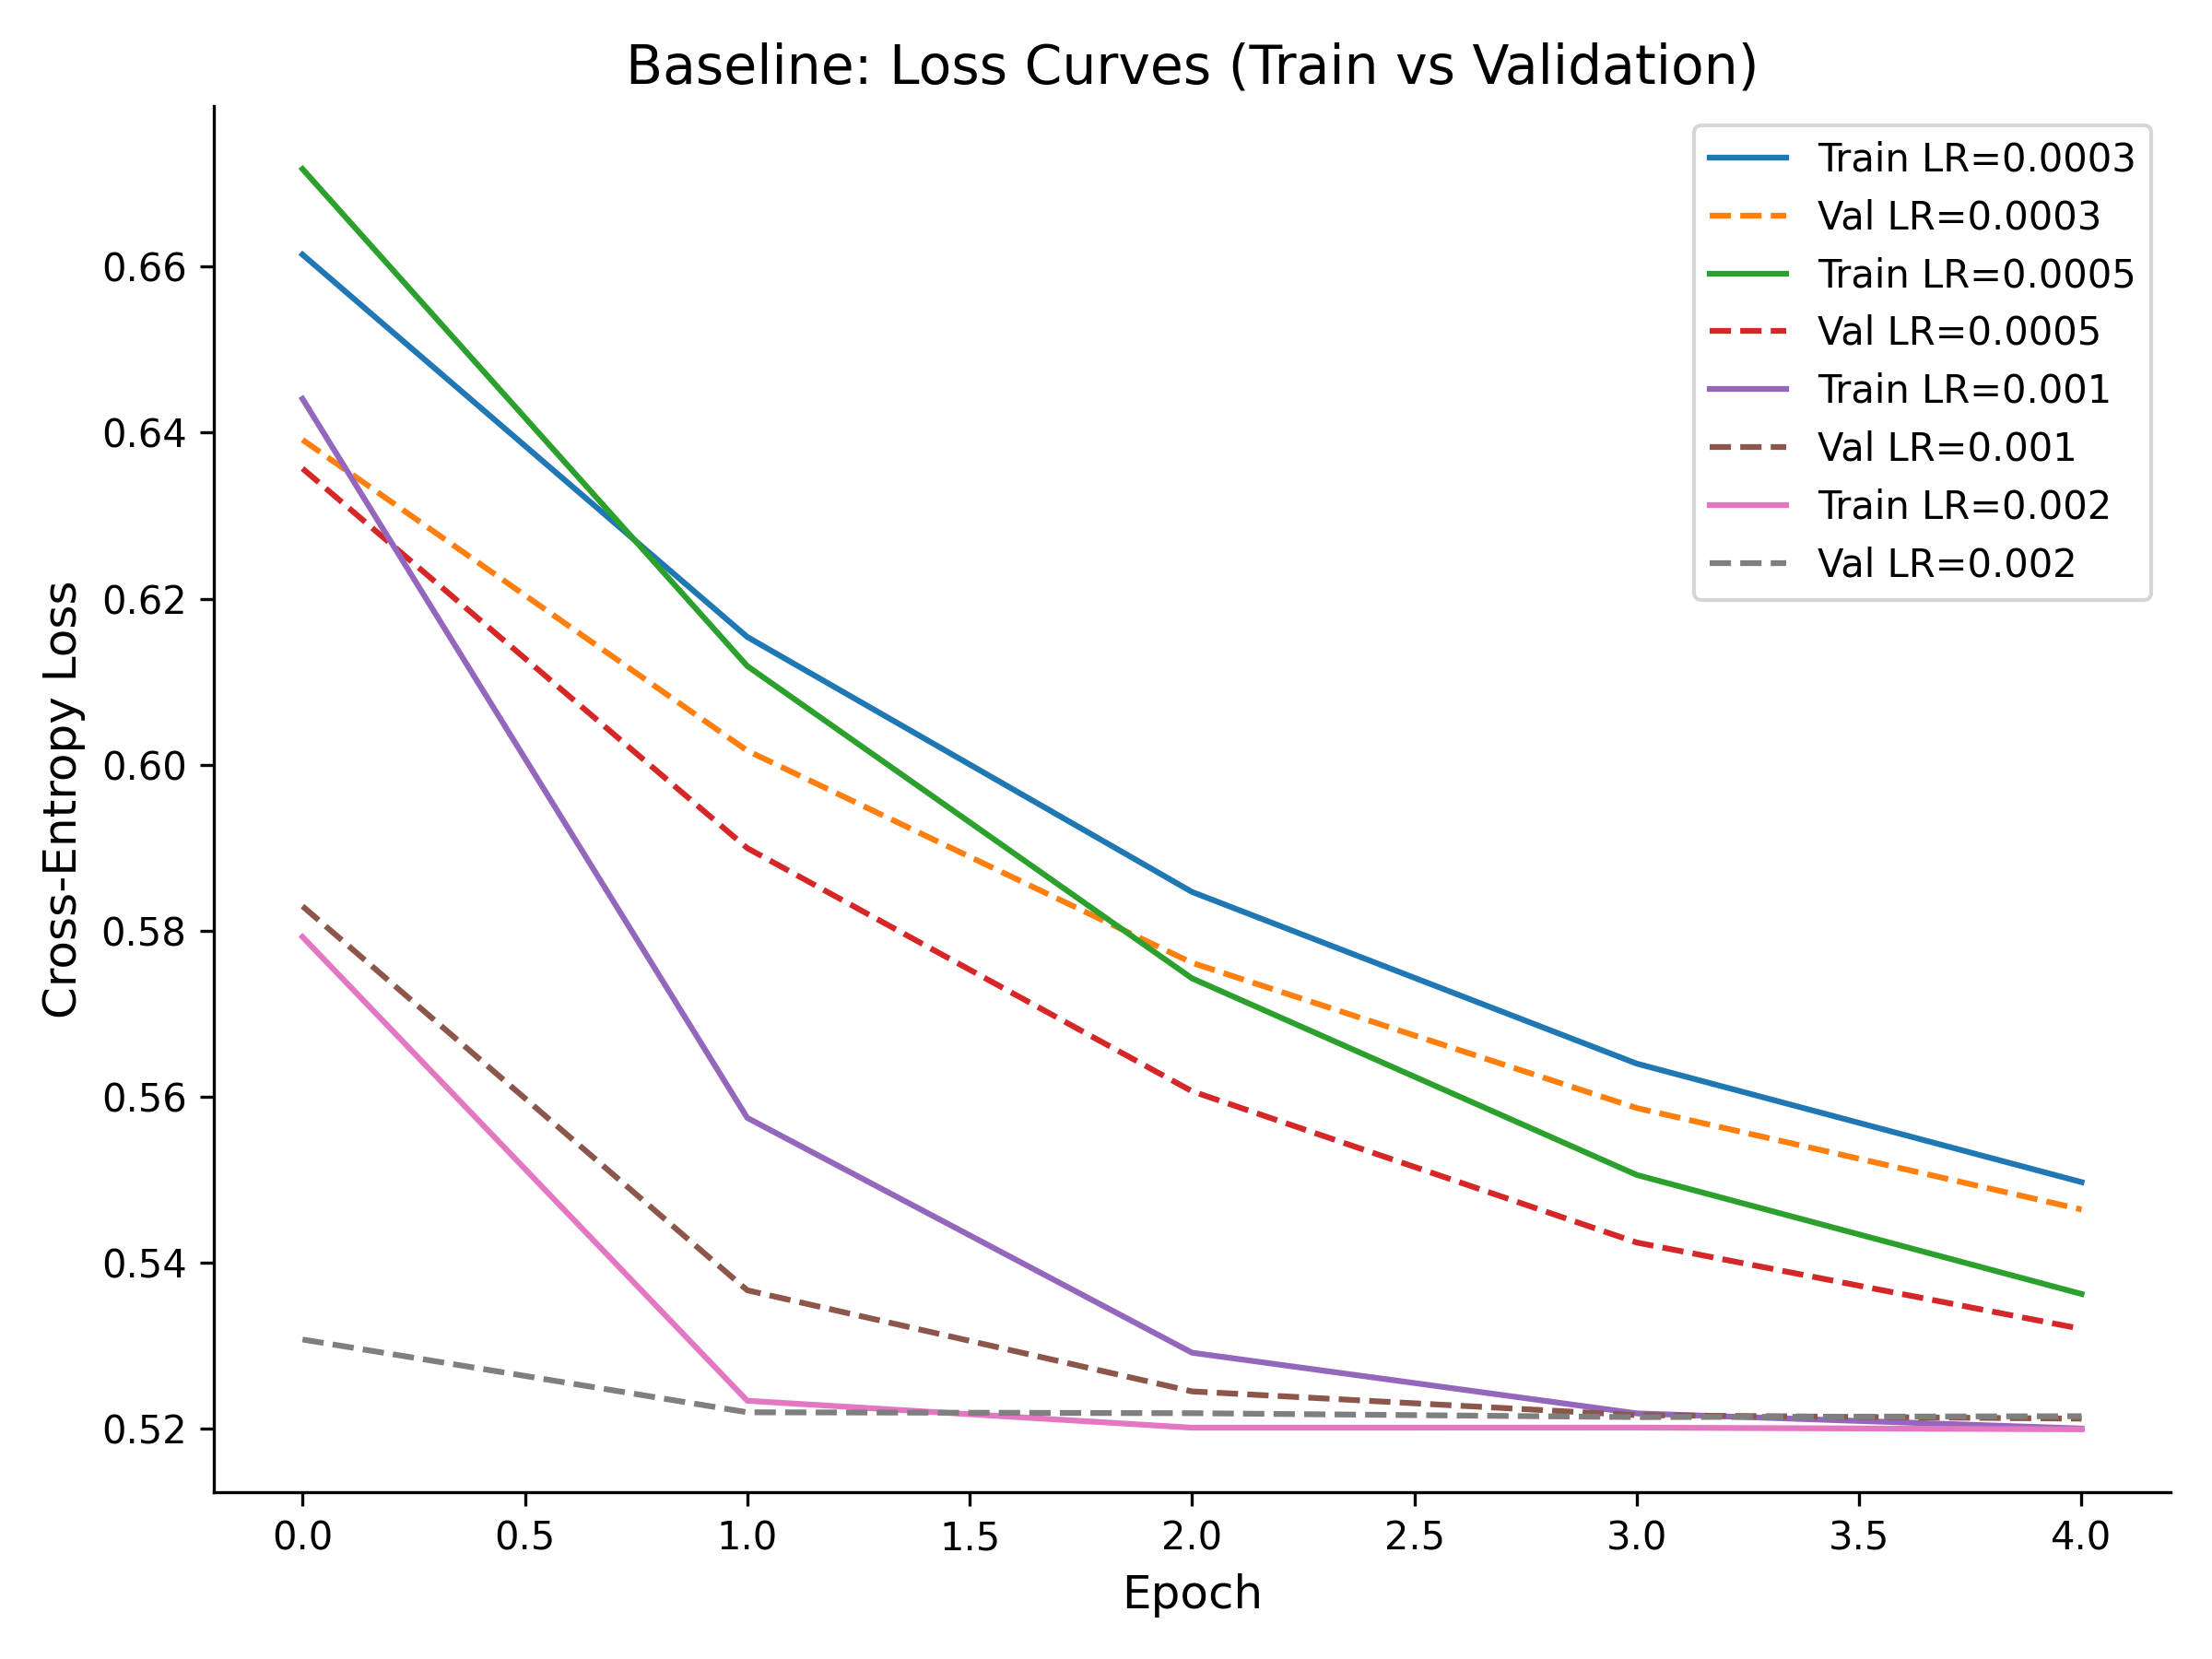
\includegraphics[width=0.45\textwidth]{baseline_loss_curves.png}
\caption{Baseline model performance trends. (Left) Macro-F1 across epochs. (Right) Training loss curves.}
\label{fig:main1}
\end{figure}

\begin{figure}[t]
\centering
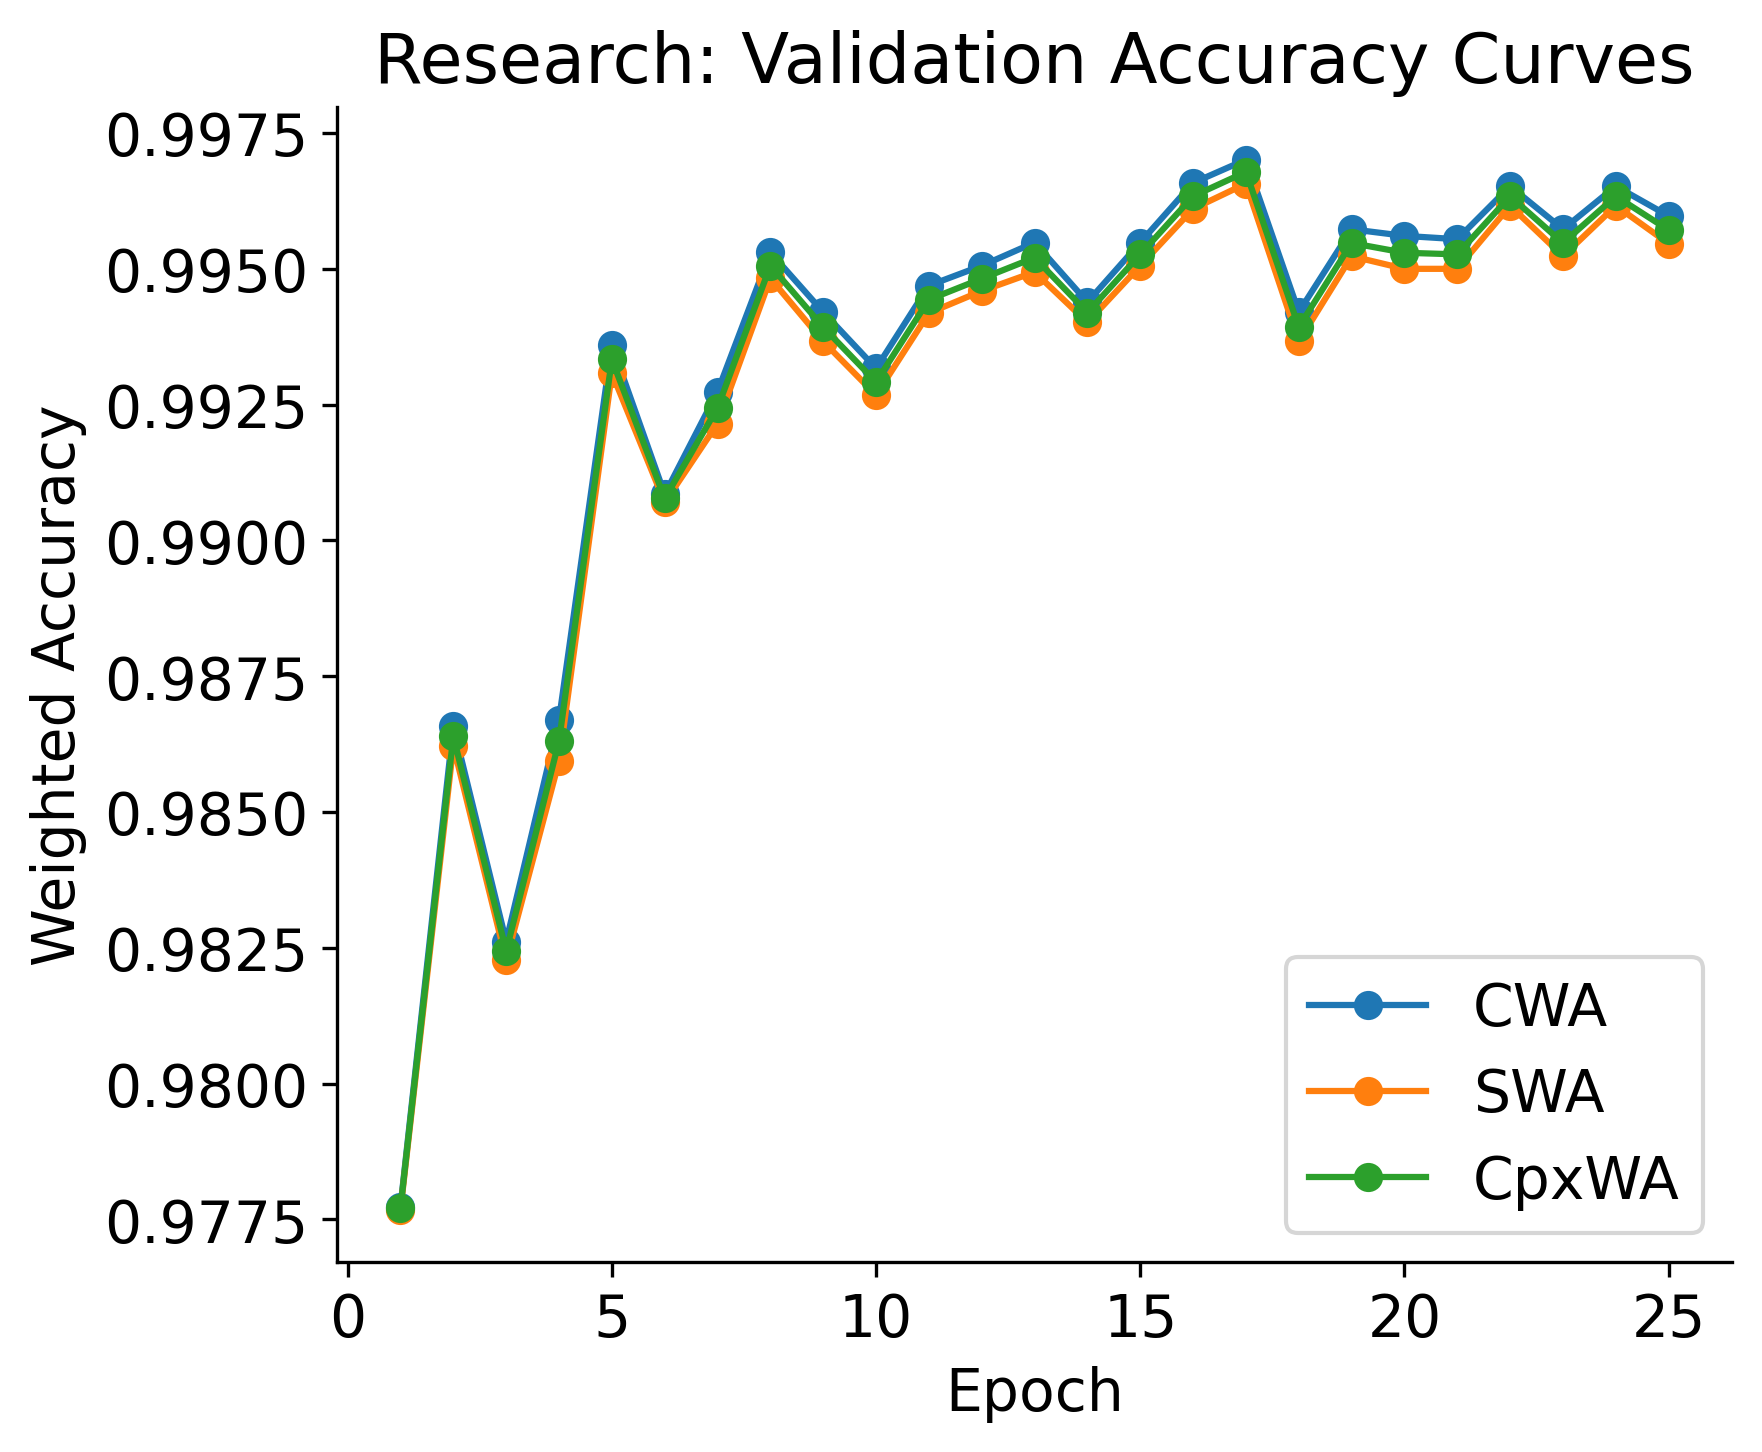
\includegraphics[width=0.45\textwidth]{research_val_metrics.png}
\hfill
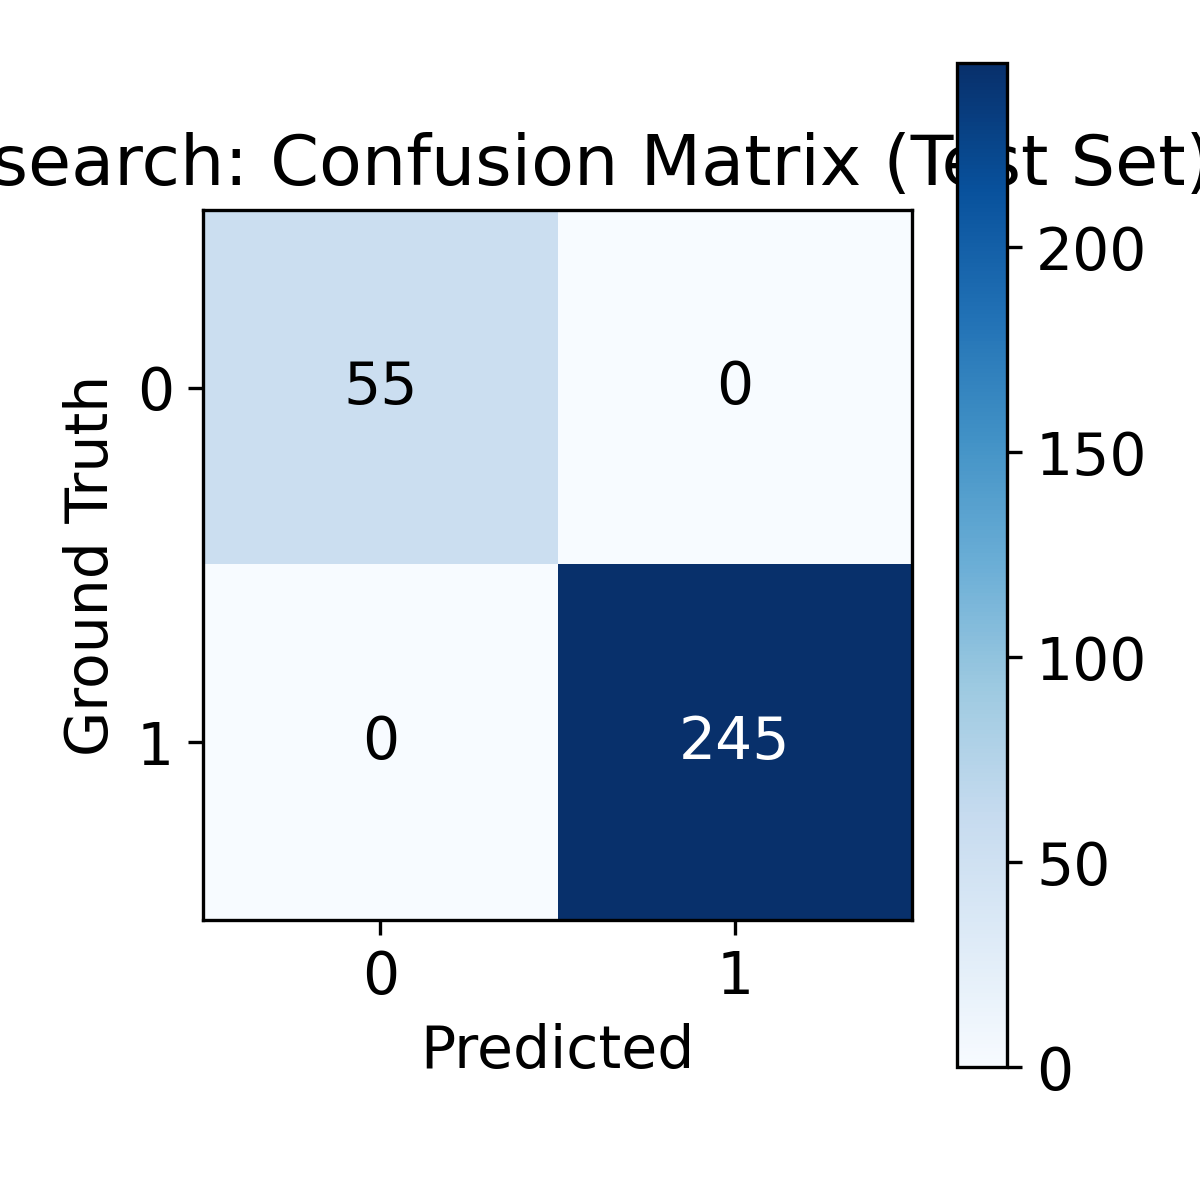
\includegraphics[width=0.45\textwidth]{research_confusion_matrix.png}
\caption{Validation metrics (left) and confusion matrix (right).}
\label{fig:main2}
\end{figure}

Ablations reveal that freezing the encoder drastically degrades final performance, removing positional embeddings skews predictions toward common classes, and excluding the projection head yields unstable training signals. Detailed ablation figures are provided in the Appendix, where each variation is juxtaposed to indicate the magnitude of performance fluctuations.

\section{Conclusion}
We highlight practical challenges encountered in neural sequence modeling despite adherence to common training practices. Key lessons include the importance of validating assumptions about pretraining data size and thoroughly testing architectural modifications. Future work will systematically dissect additional real-world pitfalls, encouraging the community to openly share unexpected or negative results that often remain overlooked.

\appendix
\section{Additional Figures and Details}
Here we present ablation plots and broader experiment logs. Each subfigure illustrates a specific architectural removal (e.g., no positional embeddings, frozen encoder) or data manipulation (e.g., reduced pretraining sets) to underscore performance variability. Comprehensive hyperparameters, training seeds, and configuration files are provided in supplementary materials.

\clearpage
\begin{filecontents}{references.bib}
@article{lecun2015,
  title={Deep learning},
  author={LeCun, Yann and Bengio, Yoshua and Hinton, Geoffrey},
  journal={Nature},
  volume={521},
  pages={436--444},
  year={2015}
}

@inproceedings{simonyan2015,
  title={Very Deep Convolutional Networks for Large-Scale Image Recognition},
  author={Simonyan, Karen and Zisserman, Andrew},
  booktitle={International Conference on Learning Representations},
  year={2015}
}

@inproceedings{vaswani2017,
  title={Attention Is All You Need},
  author={Vaswani, Ashish and Shazeer, Noam and Parmar, Niki and others},
  booktitle={Advances in Neural Information Processing Systems},
  year={2017}
}
\end{filecontents}

\bibliographystyle{plainnat}
\bibliography{references}

\end{document}